\documentclass[10pt, colorlinks=true, urlcolor=blue]{beamer}

% Themes and colors for a professional look
\usetheme{Madrid}
\usecolortheme{seagull}
\setbeamercolor{title}{fg=white,bg=blue!80!black}
\setbeamercolor{frametitle}{fg=white,bg=blue!70!black}
\setbeamercolor{block title}{fg=white,bg=blue!80!black}
\setbeamercolor{block body}{bg=blue!5!white}
\setbeamerfont{title}{size=\fontsize{12}{16}\selectfont}

% Customize the footline layout
\setbeamertemplate{footline}
{
  \leavevmode%
  \hbox{%
    % Left field (author or custom text)
    \begin{beamercolorbox}[wd=0.25\paperwidth,ht=2.5ex,dp=1ex,center]{author in head/foot}%
      \usebeamerfont{author in head/foot}\insertshortauthor
    \end{beamercolorbox}%
    % Middle field (title)
    \begin{beamercolorbox}[wd=0.5\paperwidth,ht=2.5ex,dp=1ex,center]{title in head/foot}%
      \usebeamerfont{title in head/foot}\insertshorttitle
    \end{beamercolorbox}%
    % Right field (page number)
    \begin{beamercolorbox}[wd=0.25\paperwidth,ht=2.5ex,dp=1ex,center]{date in head/foot}%
      \usebeamerfont{date in head/foot}\insertframenumber/\inserttotalframenumber
    \end{beamercolorbox}%
  }%
}

% Set hyperlink colors
\hypersetup{
    colorlinks=true,    % Enable colored links
    urlcolor=blue,      % Color for URLs
    linkcolor=blue      % Color for internal links (optional)
}

\usepackage{minted}

\title{Python `memory\_graph', quick intro}
\author{Bas Terwijn}
\titlegraphic{
\vspace{-2.8em} % Adjust this value as needed
  \makebox[\textwidth]{%
  \begin{tabular}{c c}
    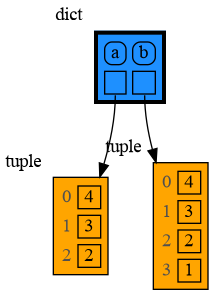
\includegraphics[height=0.35\textwidth]{figures/immutable.png} &
    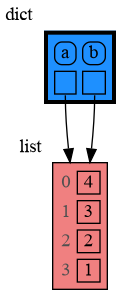
\includegraphics[height=0.35\textwidth]{figures/mutable.png} \\
      &  \\
    \multicolumn{2}{c}{
      
\includegraphics[width=0.6\textwidth]{figures/uva.png}
    }
  \end{tabular}
}
}
\date{}

\begin{document}

\begin{frame}
    \titlepage
\end{frame}

\begin{frame}{memory\_graph Debugger Setup}

  Debugger Setup
  \begin{itemize}
  \item install \href{https://pypi.org/project/memory-graph/}{\texttt{memory\_graph}} and \href{https://graphviz.org/download/}{\texttt{Graphviz}}
  \item open Python source file in Visual Studio Code and add line: \\
    \ \ \ {\footnotesize \mintinline{python}{import memory_graph as mg}}
  \item set a breakpoint, start the \href{https://code.visualstudio.com/docs/python/debugging}{\texttt{vscode debugger}} and add watch: \\
    \ \ \ {\footnotesize \mintinline{python}{mg.render(mg.stack_vscode(), 'debug.pdf')}}
  \item manually open file 'debug.pdf',  set 'Always on Top'
  \end{itemize}
  
  \vspace{1.8em}
  
  Adobe Acrobat Reader Problem: doesn't refresh and blocks updates to PDF file
  \begin{itemize}
  \item install a refreshing PDF reader: \\ \ \ \
    \href{https://www.sumatrapdfreader.org/}{\texttt{SumatraPDF}},
    \href{https://okular.kde.org/}{\texttt{Okular}}, ...
  \item or use a refreshing image viewer: \\
\ \ \ {\footnotesize \mintinline{python}{mg.render(mg.stack_vscode(), 'debug.svg')}} \\
\ \ \ {\footnotesize \mintinline{python}{mg.render(mg.stack_vscode(), 'debug.png')}}
  \end{itemize}
\end{frame}

\end{document}
